\documentclass{article}
\usepackage{textcomp}
\usepackage{tikz}
\usepackage{pgfplots}

\pgfplotsset{compat=1.9}

\begin{document}
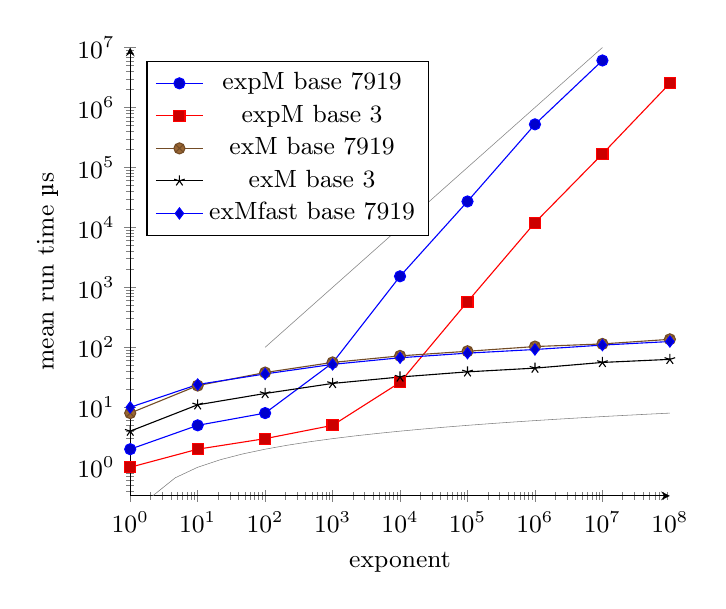
\begin{tikzpicture}

	\pgfplotsset{log base 10 number format code/.code={$10^{\pgfmathprintnumber{#1}}$}}
	\tikzstyle{every node}=[font=\small]

	\begin{loglogaxis}[
		axis x line=bottom,
		axis y line=left,
		enlarge x limits=0,
		enlarge y limits=0,
	    xlabel=exponent,
	    ylabel=mean run time \textmu s,
		legend pos=north west
	]

	\addplot plot coordinates {
	(10^0, 2)
	(10^1, 5)
	(10^2, 8)
	(1000, 55)
	(10000, 1530)
	(100000, 27105)
	(1000000, 523143)
	(10000000, 6080164)
	};

	\addplot plot coordinates {
	(10^0, 1)
	(10^1, 2)
	(10^2, 3)
	(1000, 5)
	(10000, 26)
	(100000, 576)
	(1000000, 12000)
	(10000000, 168000)
	(100000000, 2528000)
	};
	
	\addplot plot coordinates {
	(1, 8)
	(10, 23)
	(100, 38)
	(1000, 56)
	(10000, 72)
	(100000, 86)
	(1000000, 103)
	(10000000, 114)
	(100000000, 136)
	};

	\addplot plot coordinates {
	(1, 4)
	(10, 11)
	(100, 17)
	(1000, 25)
	(10000, 32)
	(100000, 39)
	(1000000, 45)
	(10000000, 56)
	(100000000, 63)
	};
	
	\addplot plot coordinates {
	(10^0, 10)
	(10^1, 24)
	(10^2, 36)
	(1000, 52)
	(10000, 67)
	(100000, 80)
	(1000000, 92)
	(10000000, 109)
	(100000000, 125)
	};
	
	\addplot[very thin,color=gray,domain=10^2:10^7] { x };
	\addplot[very thin,color=gray,domain=1:10^8] { log10(x) };

	\addlegendentry{expM base 7919}
	\addlegendentry{expM base 3}
	\addlegendentry{exM base 7919}
	\addlegendentry{exM base 3}
	\addlegendentry{exMfast base 7919}

	\end{loglogaxis}

\end{tikzpicture}
\end{document}
